\chapter{Checking \& Simulation}
\label{sec:ch5}

In this chapter, we discuss how to solve the limitations of the previous
approach and how to solve them by using the simulator.

\section{More complex specifications}
In the previous approaches is only the account specification used. In this proof
of concept, we're going to use more complex specifications, complex in the sense
that they depend and interact with each other.

We're going to use the
same account specification from \autoref{fig:account-spec}. As an addition to
account specification, we use a transaction specification. Via this
specification money can be transferred between two accounts.
The Rebel implementation of the transaction \footnote{\url{https://github.com/cwi-swat/rebel/blob/e58590c7f51f59e7ee6443bb89ef09dff6febab6/rebel-core/examples/simple_transaction/Transaction.ebl}} is shown in \autoref{fig:transaction-spec}.
As you can see the transaction specification contains more fields than the
account specification. The two remarkable fields are from and to, both are the
type of \textit{IBAN}. \textit{IBAN} is a built-in \textit{Rebel}
type.~\cite[p.~3]{stoel_storm_vinju_bosman_2016} Note that after the type
definition an annotation is given to specify a reference to another
specification, in this case, account specification. The fields to and from are
used to indicate between whom the transaction takes place.

According to the transaction specification, the transaction first
needs to be started. When a transaction is in the state validated and a booking
cannot be made, the transition \textit{fail} can be used to put the transaction in its
final state failed. To successfully complete a transaction is the transition
\textit{book} used. In comparison to the account specification, does the transaction
specification two final states, which are booked and failed. When the final
state booked or failed is reached, then there is no further action allowed.
Note that the transaction specification doesn't have an invariant.

Another difference in the transaction specification is that event definitions
can contain sync expressions. From the previous event definitions, we've only
seen pre- and postconditions. Sync expressions are used for synchronization.
These sync expressions are also translated to SMT formulas.

The sync expressions translated to the SMT solver are just logical formulas,
there is no logic for synchronization in these formulas. Of course, the generated system has
implemented synchronization for these transitions. So it is possible to also
test synchronization in the SUT. There are also several studies which reports
that SMT-based approaches to model checking can be used to test distributed
algorithms.~\cite{konnov2015you, alberti2015smt}

% Sync expressions are used to synchronously execute a blocking transition without the interference of other related transitions which may change the state of the instances used within the sync expressions. \unsure{which is better? or a paper ref?}

The \textit{book} transition uses the synchronization feature to express sync
operations (see \autoref{fig:transaction-book-event}). A sync operation is here
used to withdraw an amount from one account and to deposit to another account.

% \info{new scala generator, two-phase commit for distribution.}
% \info{explain sync stuff and about distribution, look at implementation of
% sync in smt. Theoretically it is possible to find errors in distributed stuff.}

\begin{sourcecode}[h!]
\begin{lstlisting}[]
specification Transaction {
	fields {
		id: Integer @key
		amount: Money
		from: IBAN @ref=Account
		to: IBAN @ref=Account
	}

	events {
		start[]
		book[]
		fail[]
	}

	lifeCycle {
		initial uninit -> validated: start
		validated    -> booked: book
					-> failed: fail
		final booked
		final failed
	}
}
\end{lstlisting}
\caption{Transaction specification}\label{fig:transaction-spec}
\end{sourcecode}
\FloatBarrier

\begin{sourcecode}[h!]
\begin{lstlisting}[]
event book() {
	sync {
		Account[this.from].withdraw(this.amount);
		Account[this.to].deposit(this.amount);
	}
}
\end{lstlisting}
\caption{book event definition from transaction specification}\label{fig:transaction-book-event}
\end{sourcecode}
\FloatBarrier

\section{Method}
% The simulation of Rebel is able to translate a single step to SMT formulas.

As discussed in \autoref{sec:research-method}, a model testing approach is
already done to test existing banking systems. Although, in this approach, it
was only possible to test the SUT interactively using the simulation. In this
approach are the traces from the SMT solver used to check whether the
SUT accepts the execution from the trace and whether it behaves as the
specification.~\cite[p.5]{stoel_storm_vinju_bosman_2016}

By using the traces, solves also the problems from the previous proof of
concept. With the use of traces, we know exactly which possible transitions the
SMT solver has performed and then playback these transitions in the SUT. So,
we're going to use the traces in this approach to check the behaviour of the
SUT.

\subsection{Evaluation criteria}

\subsubsection{Bugs}
In this approach we're using the traces from the SMT solver to test the SUT,
thus testing what should be possible according to the specification. The
expectation here is to find bugs in the SUT which doesn't accept the execution
from the traces.

\subsubsection{Efficiency}
By using the traces, we check whether the given execution is possible in the
SUT. Therefore, the expection is to perform the same transition from the traces
should be performed in the SUT.

\subsubsection{Coverage}
In this proof of concept is the simulation used to test transitions. Since
the simulation is able to test single steps, it is expected to test all
transitions of a specification.

\section{Approach}

\begin{figure}[h!]
  \centering
  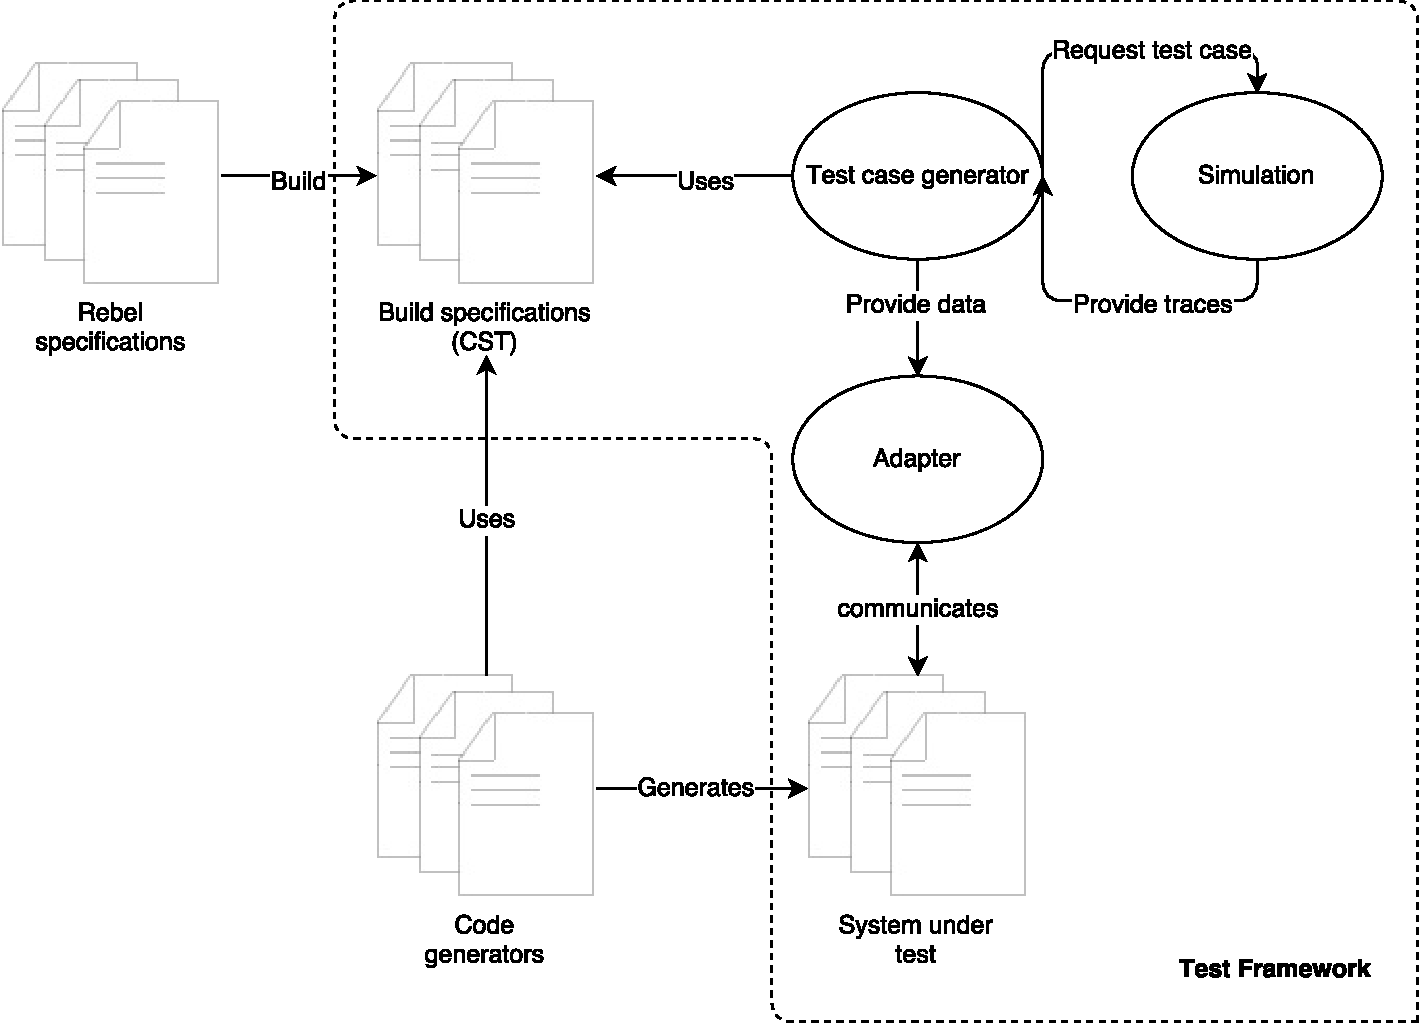
\includegraphics[width=\linewidth{}]{figures/simulation-diagram.pdf}
  \caption{Testing approach with simulation}\label{fig:simulation-testing}
\end{figure}
\FloatBarrier

To playback the steps from a given trace on the SUT, we're going to split every
transition into three steps as in the
study~\cite[p.~6]{stoel_storm_vinju_bosman_2016}:
\begin{enumerate}
\item \textbf{pre-transition check} Check whether the current state from the SUT
is conform to the current state from the trace
\item \textbf{transition check} Execute the given transition from the trace on
the SUT
\item \textbf{post-transition check} Check whether the new state from the SUT is
conform to the new state from the trace
\end{enumerate}
\unsure{paper: what is state? also the values of the instances?}

The transition function for the simulation looks as follows: $p(s_{1}, s_{2})$,
which has the pre- and postcondition of the to be executed transition
\cite[p.6]{stoel_storm_vinju_bosman_2016}. The current state $s_{1}$ holds the
constraints of the current values of the simulated specification. Hereafter, to
execute the transition the user is asked to provide the data for the transition
parameters.

Before using the simulation, two challenges needs to be solved: defining the
current state for a given transition and providing the transition parameters
data values. These challenges are discussed in the paragraphs below.

\subsection{Pre-transition check}

\subsubsection*{Current state}
\label{sec:ch5-current-state}

The pre-transition checks entail the check for the current state of the SUT is
conform to the current state from the trace. Although with the simulation it is
only possible to reason about individual steps. For some transitions a current
state is required, \textit{e.g.}, an account needs to be blocked first to
unblock it. In the simulation, a current state needs to be defined to check
whether the step can be made from the current state. This is also the case in
the SUT since a current state needs to be initialized first before the
transition is performed.

To initialize the current state in the SUT checking can be used. By defining
the current state with checking, the current state is checked and a valid trace
is given by the model checker when the current state is satisfiable. So for
every transition, a tebl needs to be generated for the state to reach
(current state) to perform the transition. Although there are a number of
caveats with the use tebl files.

When a state to reach is defined for checking, the identifiers for the entities
are only unique within that trace. For example for
\autoref{fig:tebl-opened-simple-account}, the identifier for the opened account
from the traces is \textit{NL10INGB0000001}. The identifiers for similar
entities are auto-incremented, \textit{e.g.}, when an additional account entity
is specified in \autoref{fig:tebl-opened-simple-account} the identifier is then
\textit{NL10INGB0000002}. This is not only the case with IBAN numbers, but also
with Integer, String, etc. This isn't a problem when a single transition is
tested. When multiple transitions are tested and even when there are multiple
entities, this will result in collisions of existing entities with the same
identifiers. Note also that the generated IBAN numbers by the SMT solver are
also not valid.

The invalid IBAN numbers isn't a problem for the
checking since checking is only used to reason about possible traces. However,
this doesn't hold in the SUT since SUT is a banking system and here it must
conform to the IBAN standards. It is possible with checking to define the
properties of an entity, \textit{e.g.}, the IBAN for an account.

To solve the
problem with the collision of existing entities, a random identifier should be
given for each entity. Therefore, for each type like Integer, is a simple random
generator implemented. This generator generates a random identifier which is
used as the identifier for the entities in checking. Unlike the basic types,
IBAN is a more complex type to generate since the type should conform to the
IBAN standards. Therefore, Iban4j~\cite{iban4j} is used to generate random IBAN
account numbers which are compliant to the ISO\_13616 and ISO\_9362 standards.

Another pitfall with the use of checking is the use of more complex
specifications, \textit{e.g.}, the transaction specification. With such
specifications, it is possible to have a reference to another specification. In
the case of the transaction specification involves two references, namely
account specification. To use checking in such specifications must be taken into
account the references to other specifications. Which means that for every
referencing specification in checking, imports need to be resolved and defined,
and the entity needs to be defined with an identifier. Note that these
identifiers should be again random, otherwise it will cause again collisions of
existing entities.

Altogether, a generated tebl for checking the current state looks as follows in
\autoref{fig:tebl-gen-validated-transaction}.

When the current state is defined, the generated tebl is given to the model
checker. When the current state is satisfiable are the traces used to perform
the transitions in the SUT. This is in more depth described in the section
traces. Performing each step from a trace entails the three steps to test and
perform the transition.

\begin{sourcecode}[h!]
\begin{lstlisting}[]
module simple_transaction.Test

import simple_transaction.Transaction
import simple_transaction.Account

state doCheck {
  validated Transaction with id == 65227;

  Account with accountNumber == NO3631174980518;
  Account with accountNumber == LB404150J311SB1FJV5KL1MKYAY4;
}

check doCheck reachable in max 6 steps;
\end{lstlisting}
\caption{Generated tebl for the transition book}\label{fig:tebl-gen-validated-transaction}
\end{sourcecode}
\FloatBarrier

\subsubsection*{Current state values}
After the current state is defined, the same approach from the previous chapter
can be used to check whether it satisfiable. The SMT solver returns whether the
current state is satisfiable with the traces, including the instances with its
values.

To provide transition parameters data to the simulation, is the last step taken
with its instances. The last step is taken, because the last step is the
transition which let to the current state, which is going to be used by the
simulation. The values from these instances of the simulated specifications are
given to the current state $s_{1}$.

The simulation checks only whether the step can be made from the given current
state, it doesn't check whether the current state is reachable. With the use of
checking for the current state is the current state checked whether this is
satisfiable.

\subsection{Transition check}
% Execute the given transition from the trace on the SUT

\subsubsection*{Transition parameters data values}
Since simulation is used for reasoning about individual steps, that explains why
the transition parameters data values for the chosen transition should be
provided by the user. As discussed earlier is in the model testing approach
of the study \cite[p.6]{stoel_storm_vinju_bosman_2016} chosen for interactively
using the simulation.

Manually providing the transition parameters data values
isn't relevant for us, since our intention is to test automatically the SUT.
Certainly, these values can be generated randomly, but it should satisfy the
given pre- and postconditions for the chosen transition. However, it would be
better to let the SMT solver fill these values, taking into account the pre- and
postconditions of the chosen transition. At the time of the publication of the
study~\cite{stoel_storm_vinju_bosman_2016}, this wasn't possible in the simulation, so
the simulation should be slightly modified.

In cooperation with the author of the study~\cite{stoel_storm_vinju_bosman_2016} is this feature added to the simulation.~\footnote{\url{https://github.com/cwi-swat/rebel/commit/0d29eb30a82cc5dd6d8be750daa4a24e4e2786be}}
The simulation is now able that both state variables and transition variables
can be left open, in the sense of using the expression \textit{ANY}. When the
expression \textit{ANY} is used, the SMT solver will fill in a value for the
corresponding transition parameter, satisfying the pre- and postconditions for
the chosen transition. \unsure{what about expression as iban?}

\subsubsection*{Traces}
A valid trace is a chain of valid transitions from one state to the next state
\cite[p.5]{stoel_storm_vinju_bosman_2016}. The trace may contain multiple steps,
\textit{e.g.}, to unblock an account, an account needs first to be opened and
blocked. Each step from the traces has instances with its state and values.

The instances are specific
for that step, the results after performing the step are given in the state and
values for an instance. A trace for simulation contains the state before
performing the transition, the step (transition), and then the state after
performing the step.

After everything is defined for the simulation, the simulation can test whether
it can make the single step. The simulation then works as follows
\cite[p.6]{stoel_storm_vinju_bosman_2016}:
\begin{enumerate}
\item Check whether it is possible to satisfy the contraints of the chosen
transition given the current staten and the transition parameters data values of
the event: $p(s_{1}, s_{2})$
\item Check whether the invariants hold in the state after the transition:
$P(s2)$.
\end{enumerate}

When this step can be made, with the use of traces, the step can be played in
the SUT. Therefore, \textit{JSON} should be generated for the chosen transition.
To generate this \textit{JSON} are the transition parameters data values and
the transition name read from the trace step. At last, the endpoint is
determined for the given step and is the generated JSON sent to the endpoint.

\subsection{Post-transition check}
% Check whether the new state from the SUT is conform to the new state from the trace

Since a trace contains the instances before and after the step, this can be used
in the post-transition check to test the SUT. As a result, we can check after or
before performing the step, whether the SUT behaves similarly as the
simulated/checked specification.

To check whether the new state from the SUT is
conform to the trace, the state and values from the instances are read after
performing the transition. The endpoint is then determined to retrieve the state
of these instances in the SUT. Then, the results of these instances from the SUT
and trace are compared to find any misbehaviour in the SUT.
\improvement{check all instances}

\subsubsection{Normalization}

Before a Rebel specification is checked or simulated is the specification
normalized. This normalization process is done to make the SMT formulas easier
and also to give it partially semantics
\cite[p.5]{stoel_storm_vinju_bosman_2016}. Desugaring the life cycle is part of
the normalization process. The life cycle is desugared to strengthen the pre-
and postconditions of the transitions with the life cycle information.
Therefore, are two fields added, \_state and \_step, to the fields of the
specification. To each state and event is a distinct identity assigned. The
identity of the current state is assigned to the \_state field and the identity
of the transition which led to the current state is assigned to the field
\_step. This results into that the original life cycle can be expressed, by
adding constraints on the \_state and \_step fields to the transitions pre- and
postconditions \cite[p.5]{stoel_storm_vinju_bosman_2016}.

The newly added fields
are also present within the trace from the SMT solver. In our case, we only use
the \_state field, because we already know which transition let to the current
state. To compare the current state from the \_state field, it needs to be
sugared back in order to compare it to the SUT.
% Adding Frame Conditions. To guard the fields that are not changed by the event frame conditions are added (Jack- son 2012). These frame conditions make sure that a field has the same value after the transition as before.

\subsubsection{Adapter}
As discussed in the code generation section, the request made to the API of the
SUT are "standardized", but the response isn't. For the post-transition check,
it is necessary to check the new state in the SUT, and therefore an adapter
needs to be defined to be able to compare the results of the SUT and the trace.

The decision is made to only implement an adapter for the code generator
Codegen-Akka, since this is a more mature code generator and frequently used for
experiments within ING Bank.

\info{add model checking paper for adapter}

% Using the generated test cases, we can then test the system. Usually, an adapter is used to decouple knowledge of the SUT’s external interfaces from the test generation tool. The test cases provide the inputs and expected outputs to the adapter. The adapter forwards the inputs to the SUT. When the SUT sends a response, the adapter observes it and evaluates it using the expected outputs

% as discussed with current state, all transitions contains the tree steps. It is possible that a trace can contain multiple steps, e.g. to unblock an account, an account needs first to be opened and blocked. This requires after executing each step, the step needs to be tested, in the sense of automatically repeating the process.

\section{Results}

\subsection{Codegen-Akka}

The results of the test run is shown in
\autoref{fig:ch5-res-codegenakka-account} and
\autoref{fig:ch5-res-codegenakka-transaction}. From this result, we can conclude
that the test for the close transition has failed.

\begin{table}[h!]
\centering
\begin{tabular}{ccc}
\toprule
\textbf{Transition to test} & \textbf{Current state} & \textbf{Transition} \\ \midrule
openAccount                 & \cmark{}               & \cmark{}            \\
withdraw                    & \cmark{}               & \cmark{}            \\
deposit                     & \cmark{}               & \cmark{}            \\
interest                    & \cmark{}               & \cmark{}            \\
block                       & \cmark{}               & \cmark{}            \\
unblock                     & \cmark{}               & \cmark{}            \\
close                       & \cmark{}               & \xmark{}            \\ \bottomrule
\end{tabular}
\caption{Results: testing account specification transitions}\label{fig:ch5-res-codegenakka-account}
\end{table}
\FloatBarrier

\begin{table}[h!]
\centering
\begin{tabular}{ccc}
\toprule
\textbf{Transition to test} & \textbf{Current state} & \textbf{Transition} \\ \midrule
start                       & \cmark{}               & \cmark{}            \\
book                        & \cmark{}               & \cmark{}            \\
fail                        & \cmark{}               & \cmark{}            \\ \bottomrule
\end{tabular}
\caption{Results: testing transaction specification transitions}\label{fig:ch5-res-codegenakka-transaction}
\end{table}
\FloatBarrier

\subsection{Codegen-Datomic}
The results of the test run is shown in
\autoref{fig:ch5-res-codegendatomic-account} and
\autoref{fig:ch5-res-codegendatomic-transaction}. From this result, we can
conclude again that the test for the close transition has failed. Remarkable is
that also the interest transition has failed.

\begin{table}[h!]
\centering
\begin{tabular}{ccc}
\toprule
\textbf{Transition to test} & \textbf{Current state} & \textbf{Transition} \\ \midrule
openAccount                 & \cmark{}               & \cmark{}            \\
withdraw                    & \cmark{}               & \cmark{}            \\
deposit                     & \cmark{}               & \cmark{}            \\
interest                    & \cmark{}               & \xmark{}            \\
block                       & \cmark{}               & \cmark{}            \\
unblock                     & \cmark{}               & \cmark{}            \\
close                       & \cmark{}               & \xmark{}            \\ \bottomrule
\end{tabular}
\caption{Results: testing account specification transitions}\label{fig:ch5-res-codegendatomic-account}
\end{table}
\FloatBarrier

\begin{table}[h!]
\centering
\begin{tabular}{ccc}
\toprule
\textbf{Transition to test} & \textbf{Current state} & \textbf{Transition} \\ \midrule
start                       & \cmark{}               & \cmark{}            \\
book                        & \cmark{}               & \cmark{}            \\
fail                        & \cmark{}               & \cmark{}            \\ \bottomrule
\end{tabular}
\caption{Results: testing transaction specification transitions}\label{fig:ch5-res-codegendatomic-transaction}
\end{table}
\FloatBarrier

\subsection{Codegen-Scala-ES}
The results of the test run is shown in
\autoref{fig:ch5-res-codegendatomic-account} and
\autoref{fig:ch5-res-codegendatomic-transaction}. Again the test for the
transition close has failed, but also for the transition interest.

\begin{table}[h!]
\centering
\begin{tabular}{ccc}
\toprule
\textbf{Transition to test} & \textbf{Current state} & \textbf{Transition} \\ \midrule
openAccount                 & \cmark{}               & \cmark{}            \\
withdraw                    & \cmark{}               & \cmark{}            \\
deposit                     & \cmark{}               & \cmark{}            \\
interest                    & \cmark{}               & \xmark{}            \\
block                       & \cmark{}               & \cmark{}            \\
unblock                     & \cmark{}               & \cmark{}            \\
close                       & \cmark{}               & \xmark{}            \\ \bottomrule
\end{tabular}
\caption{Results: testing account specification transitions}\label{fig:ch5-res-codegenscalaes-account}
\end{table}
\FloatBarrier

\begin{table}[h!]
\centering
\begin{tabular}{ccc}
\toprule
\textbf{Transition to test} & \textbf{Current state} & \textbf{Transition} \\ \midrule
start                       & \cmark{}               & \cmark{}            \\
book                        & \cmark{}               & \cmark{}            \\
fail                        & \cmark{}               & \cmark{}            \\ \bottomrule
\end{tabular}
\caption{Results: testing transaction specification transitions}\label{fig:ch5-res-codegenscalaes-transaction}
\end{table}
\FloatBarrier

\section{Analyse}

\subsection{Codegen-Akka}
The proof of concept uses in this test run the Codegen-Akka generator.
Investigating the test run, it seems to be that all transitions are tested
successfully, except the transition \textit{close}. Also, there seems to be a
limitation in testing the state of a specification.

\subsubsection{Close transition}
\label{sec:close-no-test-codegenakka}

The result of \textit{close} transition test is shown in
\autoref{fig:result-codegenakka-close}. As you can see on line number 28 is
constructing the current state for the close transition successful. Then the
simulation is asked to simulate the close transition, but according to the
traces of the simulation, the simulation wasn't able to make the step and the
simulation returns only the state before the transition.

\begin{sourcecode}[h!]
\begin{lstlisting}[]
Test transition close
opened -> close -> closed

0:
  now = 14 Aug 2017, 13:49

  instance: simple_transaction.Account, key = FO9402337176862639
    ?
    ?
    var accountNumber (type: IBAN) (uninitialized)
    var balance (type: Money) (uninitialized)

1:
  now = 14 Aug 2017, 13:49
  step: simple_transaction.Account.openAccount
    var initialDeposit (type: Money) = EUR50.00
    Transition to state = opened
    Identified by accountNumber = FO9402337176862639

  instance: simple_transaction.Account, key = FO9402337176862639
    State = opened
    ?
    var accountNumber (type: IBAN) = FO9402337176862639
    var balance (type: Money) = EUR50.00

Endpoint: /Account/FO9402337176862639/OpenAccount
JSON payload: { "OpenAccount": { "initialDeposit":"EUR 50.00" } }
Response: ("body":"CommandSuccess(OpenAccount(50.00 EUR))","isSuccessful":"true","message":"OK",
"errorBody":"","code":"200")

1:
  now = 12 Jul 2016, 12:00:00

  instance: simple_transaction.Account, key = FO9402337176862639
    State = opened
    ?
    var accountNumber (type: IBAN) = FO9402337176862639
    var balance (type: Money) = EUR50.00
\end{lstlisting}
\caption{No test generated for close transition}\label{fig:result-codegenakka-close}
\end{sourcecode}
\FloatBarrier

As discussed earlier, the precondition of the close transition is that there
should be no remaining balance as shown in \autoref{fig:account-close-event}.
On line number 15 of the test run is shown that the simulation makes the step to
open an account with a balance of 50 euros. Afterwards are no transitions
performed. Thus this current state does not satisfy the precondition of the
close transition. That's why the simulation wasn't able to perform the
transition since the given values from the current state to $s_{1}$ weren't
satisfying for $s_{2}$.

The generated tebl for the current state is shown in
\autoref{fig:tebl-gen-validated-transaction}. Only the state to reach is
specified with the identifier of the account. As we've seen the event definition
of \textit{openAccount} in \autoref{fig:account-openaccount-event}, the account
must be opened with a balance of 50 euros.

To conclude, the simulation wasn't able to test the transition close since the
precondition of this transition isn't satisfied in the postcondition of $s_{1}$.
This holds also for testing other generators.

\begin{sourcecode}[h!]
\begin{lstlisting}[]
module simple_transaction.Test

import simple_transaction.Account

state doCheck {
  opened Account with accountNumber == AD3517248539N3OTXZIDF13H;
}

check doCheck reachable in max 6 steps;
\end{lstlisting}
\caption{Generated tebl for the transition book}\label{fig:tebl-gen-validated-transaction}
\end{sourcecode}
\FloatBarrier

\subsubsection{State testing}

In \autoref{fig:result-not-found-state} is the test run shown of the transition
\textit{book}. Only the first transition is shown in this figure. As you can
see on line 42 is the \textit{openAccount} transition performed. On the line
below is shown that the request is successful. On line 44 is an error message
shown which tells that it isn't able to find the state of the opened account.
Note the question mark in this message. This error message is part of the
post-transition check where the new state of the SUT is tested. On line number
35 is the instance account shown after the transition and on the line below you
can see the same question mark. Both question mark relates to each other, which
is the state of a given specification.

In testing single specifications, \textit{e.g.}, in
\autoref{fig:result-codegenakka-close}, we've seen that the state is present
from the result of the SMT solver. In this case, the model checker/simulation
doesn't return the state when multiple instances are involved. So this also
happens in the \textit{start} and \textit{fail} transitions.

\begin{sourcecode}[h!]
\begin{lstlisting}[]
Test transition book
validated -> book -> booked

0:
  now = 15 Aug 2017, 11:17
  instance: simple_transaction.Transaction, key = 97691
    ?
    ?
    var id (type: Integer) (uninitialized)
    var from (type: IBAN) (uninitialized)
    var amount (type: Money) (uninitialized)
    var to (type: IBAN) (uninitialized)

  instance: simple_transaction.Account, key = CY4945493642LWV6W6RZ3EDZSGTB
    ?
    ?
    var accountNumber (type: IBAN) (uninitialized)
    var balance (type: Money) (uninitialized)

  instance: simple_transaction.Account, key = NL60IZNV8233056080
    ?
    ?
    var accountNumber (type: IBAN) (uninitialized)
    var balance (type: Money) (uninitialized)

1:
  now = 15 Aug 2017, 11:17
  step: simple_transaction.Account.openAccount
    var initialDeposit (type: Money) = EUR50.00
    Transition to state = opened
    Identified by accountNumber = NL60IZNV8233056080

  // ... other instances from the state above

  instance: simple_transaction.Account, key = NL60IZNV8233056080
    ?
    ?
    var accountNumber (type: IBAN) = NL60IZNV8233056080
    var balance (type: Money) = EUR50.00

Endpoint: /Account/NL60IZNV8233056080/OpenAccount
JSON payload: { "OpenAccount": { "initialDeposit":"EUR 50.00" } }
Response: ("body":"CommandSuccess(OpenAccount(50.00 EUR))","isSuccessful":"true","message":"OK","errorBody":"","code":"200")
Could not find state ?, expected  "state":{"?":{}}
\end{lstlisting}
\caption{State not found for entities}\label{fig:result-not-found-state}
\end{sourcecode}
\FloatBarrier

% https://github.com/ING-CoreBank-University/ing-codegen-datomic/commit/4ebcd4df0a90fc10451562a6a43c3fcd8891fce3
\subsection{Codegen-Datomic}\label{sec:bug-interest-javadatomic}

In this test run is the Javadatomic generator used. After investigating the test
run, it seems to be that testing the transition interest fails. As you can see
in \autoref{fig:result-javadatomic-interest} on line number 55, the request made
for interest transition isn't successful and the HTTP status code returned 400
is returned. Constructing the current state for the interest transition seems to
be successful (see line number 28). According to the simulation, on line number
40, the step interest is made with a negative percentage (- 7709). On line
number 47, you can see the instance after performing the interest step, which
resulted into an account entity with the state opened and with a negative
balance. To conclude, the transition interest is possible according to the
simulation.

Although, the request made for the transition interest isn't
successful, and when we take a look at the account in the SUT, the account looks
as follows in \autoref{fig:interest-opened-account-json}. The state of the
account is still opened and the balance seems to be the same when the account
was opened. From looking at the state of the account, the interest transition
isn't performed in the SUT and the state of the account is the same as before
performing the transition.

% less than percentage

\begin{sourcecode}[h!]
\begin{lstlisting}[]
Test transition interest
opened -> interest -> opened

0:
  now = 13 Jul 2017, 12:26

  instance: simple_transaction.Account, key = MD14FLBLJOYGVJMDUZVKLU4C
    ?
    ?
    var accountNumber (type: IBAN) (uninitialized)
    var balance (type: Money) (uninitialized)

1:
  now = 13 Jul 2017, 12:26
  step: simple_transaction.Account.openAccount
    var initialDeposit (type: Money) = EUR50.00
    Transition to state = opened
    Identified by accountNumber = MD14FLBLJOYGVJMDUZVKLU4C

  instance: simple_transaction.Account, key = MD14FLBLJOYGVJMDUZVKLU4C
    State = opened
    ?
    var accountNumber (type: IBAN) = MD14FLBLJOYGVJMDUZVKLU4C
    var balance (type: Money) = EUR50.00

Endpoint: /Account/MD14FLBLJOYGVJMDUZVKLU4C/OpenAccount
JSON payload: { "OpenAccount": { "initialDeposit":"EUR 50.00" } }
Response: ("body":"{\"iban\":\"MD14FLBLJOYGVJMDUZVKLU4C\"}","isSuccessful":"true","message":"OK",
"errorBody":"","code":"200")

1:
  now = 12 Jul 2016, 12:00:00

  instance: simple_transaction.Account, key = MD14FLBLJOYGVJMDUZVKLU4C
    State = opened
    ?
    var accountNumber (type: IBAN) = MD14FLBLJOYGVJMDUZVKLU4C
    var balance (type: Money) = EUR50.00

2:
  now = 12 Jul 2016, 12:00:00
  step: simple_transaction.Account.interest
    var currentInterest (type: Percentage) = (- 7709)
    Transition to state = opened
    Identified by accountNumber = MD14FLBLJOYGVJMDUZVKLU4C

  instance: simple_transaction.Account, key = MD14FLBLJOYGVJMDUZVKLU4C
    State = opened
    ?
    var accountNumber (type: IBAN) = MD14FLBLJOYGVJMDUZVKLU4C
    var balance (type: Money) = - EUR3804.50

Endpoint: /Account/MD14FLBLJOYGVJMDUZVKLU4C/Interest
JSON payload: { "Interest": { "currentInterest":"-77.09" } }
Response: ("body":"","isSuccessful":"false","message":"Bad Request","errorBody":"","code":"400")
\end{lstlisting}
\caption{Failing test on interest transition with the use of javadatomic generator}\label{fig:result-javadatomic-interest}
\end{sourcecode}
\FloatBarrier

\begin{sourcecode}[h!]
\begin{lstlisting}[]
{
	"_id": 17592186045441,
	"_version": 1,
	"_status": "OPENED",
	"accountNumber": {
		"iban": "MD14FLBLJOYGVJMDUZVKLU4C"
	},
	"balance": {
		"value": 50.00,
		"currency": "EUR"
	}
}
\end{lstlisting}
\caption{Account state in the SUT after performing the interest transition}
\label{fig:interest-opened-account-json}\end{sourcecode}
\FloatBarrier

The event definition for the interest transition is given in
\autoref{fig:account-interest-event}. This event definition states that the
precondition is that the \textit{currentInterest} must be less than or equal
10\%, and the postcondition is that the balance must be changed after applying
the interest. The generated transition parameter \textit{currentInterest},
- 7709, satisfies also this precondition.

\begin{sourcecode}[h!]
\begin{lstlisting}[]
function singleInterest(balance: Money, interest: Percentage): Money =  balance * interest;

event interest[maxInterest: Percentage = 10%](currentInterest: Percentage) {
  preconditions {
    currentInterest <= maxInterest;
  }
  postconditions {
    new this.balance == this.balance + singleInterest(this.balance, currentInterest);
  }
}
\end{lstlisting}
\caption{interest event definition from account specification}\label{fig:account-interest-event}
\end{sourcecode}
\FloatBarrier

Now we know that we've discovered a bug, since the simulated transition is
conform to the specification, we want to know where this misbehaviour occurs and
which code isn't correctly generated. The generated code for the interest event
definition from \autoref{fig:account-interest-event} contains the following
check in \autoref{fig:java-gen-interest-pre}. The generated code for the
preconditions seems to be good since it uses a \textit{isLessOrEqualThan}
function with the given interest percentage. Looking at the log file created by
the SUT, the exception \textit{BuildCASTransactionException} is thrown when
performing the interest transition, which is the exception from
\autoref{fig:java-gen-interest-pre}. So the generated code seems to be good, but
the function used for validating the interest returns an inappropriate value,
which lets to throw the exception.

\begin{sourcecode}[h!]
\begin{lstlisting}[language=Java]
if(! (isLessOrEqualThan(currentInterest, 10 /* % */))) {
  throw new BuildCASTransactionException("Predicate did not hold: InterestTransaction: currentInterest <= 10%");
}
\end{lstlisting}
\caption{Code in Java}\label{fig:java-gen-interest-pre}
\end{sourcecode}
\FloatBarrier

The function \textit{isLessOrEqualThan} is shown in
\autoref{fig:java-less-or-equal-check}. This function takes two parameters, both
of the type \textit{BigDecimal}, and compares the \textit{lhs} to the
\textit{rhs}, this result should be greater or equal than zero. This function
isn't correctly defined, since this is the definition for the function
\textit{isGreaterOrEqualThan}. This code isn't generated but is part of the
fixed code.

Clearly, we've discovered a bug in the SUT for the transition
interest. As discussed in \autoref{sec:ch3-evalution}, it is possible to have
bugs in the fixed code. With this proof of concept and testing the javadatomic
generator, we can conclude that we've found a bug in the fixed code.

\begin{sourcecode}[h!]
\begin{lstlisting}[language=Java]
public static boolean isLessOrEqualThan(BigDecimal lhs, BigDecimal rhs) {
  return lhs.compareTo(rhs) >= 0;
}
\end{lstlisting}
\caption{Code in Java}\label{fig:java-less-or-equal-check}
\end{sourcecode}
\FloatBarrier

\subsection{Codegen-Scala-ES}
\label{sec:bug-interest-scalaes}
% Interest squants dimensionlessdata

This test run tests the SUT generated by the Scala-ES generator. Looking at the
test run, just like the test run for the Javadatomic generator, it seems to be
that the transition interest fails. The results of the test run are shown in
\autoref{fig:result-scalaes-interest}. Line number 51 shows the failing request
for the interest transition, an error message is returned with the HTTP status
code 400. Also, in this test run is construction the current state for the
interest transition successful (see line number 26). In this test run has the
simulation generated the same trace for the interest transition as for the
Javadatomic generator. The state of the account in the SUT looks as follows in
\autoref{fig:interest-opened-account-scalaes-json}. Also here is the state of the
account opened and the balance seems to be the same when the account was opened.
So, the performed interest transition has failed and is the state of the account
the same before performing the transition.

\begin{sourcecode}[h!]
\begin{lstlisting}[]
Test transition interest
opened -> interest -> opened

0:
  now = 12 Aug 2017, 18:29
  instance: simple_transaction.Account, key = MT58PDLQ09015VOS06LIF4Q525NRO1I
    ?
    ?
    var accountNumber (type: IBAN) (uninitialized)
    var balance (type: Money) (uninitialized)
1:
  now = 12 Aug 2017, 18:29
  step: simple_transaction.Account.openAccount
    var initialDeposit (type: Money) = EUR50.00
    Transition to state = opened
    Identified by accountNumber = MT58PDLQ09015VOS06LIF4Q525NRO1I

  instance: simple_transaction.Account, key = MT58PDLQ09015VOS06LIF4Q525NRO1I
    State = opened
    ?
    var accountNumber (type: IBAN) = MT58PDLQ09015VOS06LIF4Q525NRO1I
    var balance (type: Money) = EUR50.00

Endpoint: /Account/MT58PDLQ09015VOS06LIF4Q525NRO1I/OpenAccount
JSON payload: { "OpenAccount": { "initialDeposit":"EUR 50.00" } }
Response: ("body":"{\"iban\":\"MT58PDLQ09015VOS06LIF4Q525NRO1I\"}","isSuccessful":"true",
"message":"OK","errorBody":"","code":"200")

1:
  now = 12 Jul 2016, 12:00:00
  instance: simple_transaction.Account, key = MT58PDLQ09015VOS06LIF4Q525NRO1I
    State = opened
    ?
    var accountNumber (type: IBAN) = MT58PDLQ09015VOS06LIF4Q525NRO1I
    var balance (type: Money) = EUR50.00
2:
  now = 12 Jul 2016, 12:00:00
  step: simple_transaction.Account.interest
    var currentInterest (type: Percentage) = (- 7709)
    Transition to state = opened
    Identified by accountNumber = MT58PDLQ09015VOS06LIF4Q525NRO1I

  instance: simple_transaction.Account, key = MT58PDLQ09015VOS06LIF4Q525NRO1I
    State = opened
    ?
    var accountNumber (type: IBAN) = MT58PDLQ09015VOS06LIF4Q525NRO1I
    var balance (type: Money) = - EUR3804.50

Endpoint: /Account/MT58PDLQ09015VOS06LIF4Q525NRO1I/Interest
JSON payload: { "Interest": { "currentInterest":"-77.09" } }
Response: ("body":"","isSuccessful":"false","message":"Bad Request",
"errorBody":"com.fasterxml.jackson.databind.JsonMappingException: Can not construct instance of
squants.Dimensionless: no String-argument constructor&#x2F;factory method to deserialize from String
value (&#x27;-77.09&#x27;)\n at [Source: io.undertow.servlet.spec.ServletInputStreamImpl@578015db;
line: 1, column: 35] (through reference chain: nl.ing.corebank.dto.
account.Interest[&quot;currentInterest&quot;])","code":"400")
\end{lstlisting}
\caption{Failing test on interest transition with the use of Scala-ES generator}\label{fig:result-scalaes-interest}
\end{sourcecode}
\FloatBarrier

\begin{sourcecode}[h!]
\begin{lstlisting}[]
{
   "_id":"nl.ing.corebank.aggregates.AccountAggregate$|077708cd-769a-48ec-8006-d607241c4f45",
   "_version":1,
   "_state":"OpenedState",
   "accountNumber":{
      "iban":"MT58PDLQ09015VOS06LIF4Q525NRO1I"
   },
   "balance":"50.00 EUR"
}
\end{lstlisting}
\caption{Account state in the SUT after performing the interest transition}\label{fig:interest-opened-account-scalaes-json}
\end{sourcecode}
\FloatBarrier

Likewise, the Javadatomic generator, we've discovered a bug in the SUT, since
the simulated transition isn't conform to the specification. To know where this
bug occurs and which code isn't properly generated, the response from the
interest transition request gives an error message. According to the error
message, the SUT isn't able to construct the instance of \textit{Dimensionless}
for the transition parameter \textit{currentInterest}. This error seems to occur
in the class \textit{Interest}, which is shown in
\autoref{fig:scala-gen-interest-json}. The parameter \textit{currentInterest}
indeed uses the type \textit{Dimensionless} here.

\begin{sourcecode}[h!]
\begin{lstlisting}[language=scala]
@JsonRootName(value = "Interest")
@JsonCreator
case class Interest(@JsonProperty("currentInterest") currentInterest: Dimensionless)
\end{lstlisting}
\caption{Code in Scala}\label{fig:scala-gen-interest-json}
\end{sourcecode}
\FloatBarrier

The class from \autoref{fig:scala-gen-interest-json} is used in
\autoref{fig:scala-gen-interest-request}. The \textit{interest} method handles
the interest transition and as you can see is the class \textit{Interest} used
as the second parameter. This class is used to bind the interest parameter as a
type of the \textit{Interest} class.

In short, we've discovered a bug in the SUT
for the interest transition. The interest transition bug in the Javadatomic
generator belongs to the fixed code category, but in this case, for the Scala-ES
generator, the bug belongs to the injected code category, since the
\textit{Interest} class is generated and injected in the generated code.

\begin{sourcecode}[h!]
\begin{lstlisting}[language=scala]
@POST
@Consumes(Array[String](MediaType.APPLICATION_JSON))
@Produces(Array[String](MediaType.APPLICATION_JSON))
@Path("/{accountNumber}/Interest")
def interest(@Suspended asyncResponse: AsyncResponse,
  @PathParam("accountNumber") accountNumber: IBAN, interest: Interest): Unit = {
\end{lstlisting}
\caption{Code in Scala}\label{fig:scala-gen-interest-request}
\end{sourcecode}
\FloatBarrier

% \subsection{Two-phase commit}
% datetime transaction

\section{Evaluation}\label{sec:ch5-evaluation}

\subsection{Bugs}
The expection for the criteria bugs from \autoref{sec:ch5-eval-criteria} is to
find bugs in the SUT where execution traces from the SMT solver isn't accepted
by the SUT.

In this proof of concept we've found bugs in the code generators. For both bugs,
\autoref{sec:bug-interest-javadatomic} and \autoref{sec:bug-interest-scalaes},
it wasn't possible to perform the execution from the traces returned by the
SMT solver. To conclude, we did find bugs as expected where the SUT wasn't
conform to the specification.

\subsection{Efficiency}
With the use of traces it is expected to perform the same transition from the
traces in the SUT.

Checking and simulation are used to generate tests for transitions in this proof
of concept. The traces given by the simulation and checking are used to check
whether the SUT behaves as the specification and whether it accepts the
execution from the trace. In this proof of concept are the transitions in the
SUT performed in three steps to identify misbehaviour in the SUT.
To conclude, as expected are the same transitions from the traces performed in
the SUT.

\subsection{Coverage}
The expectation of the coverage criteria is to test all the transitions from a
specification since the simulation is able to test single steps.

With this proof of concept it isn't possible to test the
\textit{close} transition. The the precondition of this transition isn't
satisfied due to the current state defined for this transition. Altogether,
with this proof of concept it is possible to test all the
transitions when the preconditions of a given transition are satisfied by the
current state.

\section{Conclusion}
In this proof of concept are more complex specifications used for testing.
Checking and simulation are used to generate tests for transitions in this proof
of concept. The traces given by the simulation and checking are used to check
whether the SUT behaves as the specification and whether it accepts the
execution from the trace. Unlike the previous proof of concept from
\autoref{sec:ch4}, it tests what should be possible according to the
specification by using the traces from the SMT solver. Even are the transition
parameters data values generated by the SMT solver. In this proof of concept are
the transitions in the SUT performed in three steps to identify misbehaviour in
the SUT. Although there is a limitation in the testing of states. Within a
trace, not every instance may contain the state of it.
\improvement{add results for this in codegen akka}

Also with this proof of concept we've found bugs in the code generators. The bug
in the interest transition from \autoref{sec:bug-interest-javadatomic} is found
in the fixed code. Another bug for the same interest transition from
\autoref{sec:bug-interest-scalaes} belongs to the category injected code since
the bug is found in the generated code from the specification. As discussed in
\autoref{sec:ch3-evalution}, it is possible that there might be bugs in
templating, in the fixed code or the injected code. With the test run of this
proof, of concept we've found bugs for both categories.

As discussed before, with this proof of concept it wasn't possible to test the
\textit{close} transition. The the precondition of this transition isn't
satisfied due to the current state defined for this transition. To sum up, with
this proof of concept it is possible to test all the transitions when the
preconditions of a given transition are satisfied by the current state. The
theory for this proof of concept is as follows:
$\forall e s_{1} \to s_{2}, (! s_{2} pre(e) \lor s_{2} pre(e) in s_{1} post(e))$.

\info{sync expression}
\info{iban encoding}

\section{Threats to validity}

\subsection*{Limited specifications}
In the conducted experiments are the specifications account and transaction used
to test the generated system from these specifications. With these experiments
and specifications, we did find faults in the code generators. Although are
these specifications quite simple, \textit{e.g.}, for a bank these
specifications would be more complex. These experiments take into account the
generosity of specifications, but with such a large amount of complex
specifications, it is questionable whether these experiments still produce
valuable results.

\subsection*{Rebel interpretation in SMT solver}
The SMT solver can be seen as an interpreter for Rebel specifications. The
conducted experiments use the SMT solver to test the generated systems from the
specifications. We already discussed before the limitation of interpretation of
Rebel specifications, and in some cases, workarounds have been used. There may
be more unknown limitations of the interpretation of Rebel specifications, which
can cause the conducted experiments give incorrect results.

\subsection*{Valid execution trace}
The experiment from \autoref{sec:ch5} tests only valid execution traces from
the SMT solver, \textit{i.e.}, testing only what should be possible according to
the specification. Testing valid execution traces is not enough, testing not
valid execution traces can be valuable. Thus the experiment from
\autoref{sec:ch4} already does this, but as discussed it has a few limitations.
